\documentclass[11pt,letterpaper]{article}
% Compile from this directory with: pdflatex main.tex (run twice for references).
% Enter the student ID before submission.
\usepackage[margin=1in]{geometry}
\usepackage{mathptmx}
\usepackage[T1]{fontenc}
\usepackage{amsmath,amssymb}
\usepackage{setspace}
\usepackage{graphicx,float,booktabs,array}
\usepackage{caption}
\usepackage{titlesec}
\usepackage[hidelinks]{hyperref}
\onehalfspacing
\setlength{\parindent}{0pt}
\setlength{\parskip}{4pt}
\setlength{\abovedisplayskip}{5pt}
\setlength{\belowdisplayskip}{5pt}
\setlength{\abovedisplayshortskip}{3pt}
\setlength{\belowdisplayshortskip}{3pt}
\titlespacing*{\section}{0pt}{9pt}{4pt}
\titlespacing*{\subsection}{0pt}{7pt}{3pt}
\titleformat{\section}{\normalfont\large\bfseries}{\thesection}{0.6em}{}
\titleformat{\subsection}{\normalfont\normalsize\bfseries}{\thesubsection}{0.6em}{}
\captionsetup{font=small,labelfont=bf,skip=4pt}
\setlength{\textfloatsep}{6pt}
\setlength{\intextsep}{6pt}
\newcommand{\R}{\mathbf R}
\newcommand{\vect}[1]{\mathbf #1}
\newcommand{\videolink}[2]{\href{run:simulalted_environments/#1}{\texttt{#2}}}
\begin{document}
\begin{titlepage}
\centering
\vspace*{0.6in}
{\LARGE\bfseries Physics-Based Simulation of a\\[5pt]Three-Dimensional LiDAR Sensor\par}
\vspace{0.3in}
{\large MAE 5810 Robot Perception\\Midterm Project Report\par}
\vspace{0.45in}
Author: Arunkumar Venkatesan\par
\vspace{0.15in}
Student ID \rule{2.6in}{0.4pt}\par
\vspace{0.3in}
Instructor: Silvia Ferrari\par
October 20, 2026\par
\vspace{0.45in}
\textbf{Project evidence guide}\par
\vspace{0.08in}
\begin{tabular}{@{}p{1.55in}p{4.4in}@{}}\toprule
Requirement & Report evidence\\\midrule
Physical model & Section~\ref{sec:theory}; Figures~\ref{fig:fov}, \ref{fig:sensor}, and~\ref{fig:threshold}\\
Simulation procedure & Section~\ref{sec:procedure}; setup, parameters, and saved evidence\\
Dependencies and reproduction & Section~\ref{sec:procedure}; install and run commands\\
Results and media & Section~\ref{sec:results}; Figures~\ref{fig:fov}--\ref{fig:maps} and three videos\\\bottomrule
\end{tabular}\par
\vspace{0.25in}
\textbf{Companion videos}\par
{\small\setstretch{1.1}
\videolink{environment_conditions.mp4}{environment\_conditions.mp4}\\
\videolink{sensor_state_best_vs_worst.mp4}{sensor\_state\_best\_vs\_worst.mp4}\\
\videolink{sampling_reflectance_factorial.mp4}{sampling\_reflectance\_factorial.mp4}\par}
\vspace{0.15in}
{\small The three files accompany this report in \texttt{simulalted\_environments/}. Open them directly if the PDF viewer disables local media links.\par}
\end{titlepage}
\setcounter{page}{2}

\section*{Abstract}
This report develops and tests a simulated spinning, three-dimensional pulsed LiDAR used by a point-cloud navigation system. The model traces each beam to the first visible surface, estimates the return from surface response and two-way atmospheric attenuation, and then applies a noisy threshold detector and a signal-dependent range-error model. Analytic checks found no eligibility or deterministic-detection mismatches in 65 geometry cases; the maximum relative power error was $4.39\times10^{-16}$ across 72 radiometry checks. The controlled experiments vary sensor configuration, target properties, sampling density, receiver noise, and weather. Across nine closed-loop weather runs, endpoint-cell coverage fell from 73.67\% in normal air to 47.10\% in fog, although all runs reached the goal. A separate 33,000-trial threshold study produced a detection-probability calibration RMS error of 0.547 percentage points. These results check consistency with the assumptions built into the simulator; they do not establish physical LiDAR calibration or general navigation reliability.

\section{Introduction}\label{sec:introduction}
A LiDAR point cloud depends on more than where a beam is aimed. The simulator must first determine which surface the beam reaches, then decide whether the return is strong enough to be detected. A target can be inside the nominal field of view (FOV) and still produce no point because the beam pattern misses it, an opaque object blocks it, the hit falls outside the range gate, or the returned power is too weak. Once detected, points support navigation and endpoint mapping, but changes in the point cloud do not always produce visible changes in the robot's route.

The experiments address four questions: whether the geometric and power calculations agree with analytic checks; how sensor pose, sampling, target properties, and atmospheric attenuation affect measurements; whether repeated detector trials follow the assumed probability and range-noise models; and how changing measurements affects mapping and closed-loop navigation. To separate causes, the sampling--reflectance experiment replays the same recorded robot poses, the target study changes one target property at a time, and the weather study includes both matched-pose replays and independent closed-loop runs. The matched-pose comparisons isolate measurement changes, while the closed-loop runs show the combined effect of sensing and controller response.

The navigation task uses an A* route planned from a partial map. Three obstacles are withheld from the planner and can be encountered only through LiDAR returns; the local controller does not receive their labels or ground-truth geometry. The study is not a SLAM evaluation: map accumulation uses the known simulated pose, each scan is treated as a snapshot, and the model omits atmospheric backscatter, moving objects, latency, and physical-device calibration. The surface-response model is related to Heiden et al. [2], although their continuous-wave phase estimator differs from the pulsed geometric and threshold model used here. The report structure follows the course guidelines [1].

\section{Theory and Methods}\label{sec:theory}
\subsection{Scan pattern}
The sensor frame has $x$ forward, $y$ left, and $z$ up; world $z$ is up. With $M$ azimuth samples per revolution and $L$ channels,
\begin{equation}\label{eq:angles}
\alpha_i=\alpha_{\min}+\frac{2\pi i}{M},\qquad
\beta_j=\beta_{\min}+\frac{j(\beta_{\max}-\beta_{\min})}{L-1}.
\end{equation}
\begin{equation}\label{eq:beam}
\vect b_{ij}=[\cos\beta_j\cos\alpha_i,\ \cos\beta_j\sin\alpha_i,\ \sin\beta_j]^{\mathsf T}.
\end{equation}
A full sweep uses $i=0,\ldots,M-1$; a partial window selects from the same full-circle angular grid. For $L=1$, the implementation uses the upper elevation directly rather than evaluating the denominator in Equation~\eqref{eq:angles}. Equations use radians and plots use degrees.

\subsection{Pose and coverage}
All channels at one azimuth share a firing time. The generic scan model translates the origin at constant world velocity; yaw may change while roll and pitch remain fixed:
\begin{equation}\label{eq:time}
t_i=\frac{\alpha_i-\alpha_{\min}}{2\pi f_{\mathrm{rot}}},\qquad \vect o_i=\vect o_0+\vect v t_i.
\end{equation}
The rotation is $\R=R_z(\mathrm{yaw})R_y(\mathrm{pitch})R_x(\mathrm{roll})$ and world beam $\vect d=\R\vect b$. For point $\vect p$, let $\vect q=\R^{\mathsf T}(\vect p-\vect o)$, $r=\|\vect q\|$, $a=\operatorname{atan2}(q_y,q_x)$, and $e=\arcsin(q_z/r)$. The nominal FOV is
\begin{equation}\label{eq:fov}
\mathcal F=\{\vect p:r_{\min}\leq r\leq r_{\max},\ a\in\mathcal A,\ \beta_{\min}\leq e\leq\beta_{\max}\}.
\end{equation}
Here $\mathcal A$ is a circular azimuth window. Discrete beams can miss targets inside this continuous set. Each subray takes the nearest opaque intersection with scene surfaces $\mathcal S$:
\begin{equation}\label{eq:los}
r_k=\min\{s>10^{-6}\,\mathrm m:\vect o+s\vect d_k\in\mathcal S\}.
\end{equation}
The simulator resolves the first surface hit before applying the range gate. As a result, even a weak or too-near object can occlude a farther surface. For finite beams, it samples subrays in the plane normal to the central direction and assigns normalized Gaussian weights. The angular standard deviation is one quarter of the full divergence $\delta$, and sunflower offsets are limited to 2.5 standard deviations. The navigation experiments use one subray per beam and snapshot poses, so motion during a scan is not modeled.

\subsection{Surface power and echo formation}
For surface normal $\vect n$, $\mu=\max(0,-\vect n^{\mathsf T}\vect d)$. Diffuse weight $\rho_d$, specular weight $\rho_s$, and exponent $m$ define
\begin{equation}\label{eq:brdf}
f=\frac{\rho_d}{\pi}+\frac{\rho_s(m+2)}{2\pi}[\max(2\mu^2-1,0)]^m.
\end{equation}
\begin{equation}\label{eq:power}
P_k=w_kP_tA_r\eta f\frac{\mu_k}{r_k^2}\exp(-2\kappa r_k).
\end{equation}
The $1/r^2$ term accounts for inverse-square spreading, while $\exp(-2\kappa r)$ represents attenuation on the outward and return paths. The receiver aperture is $A_r=\pi(D_r/2)^2$, and $\eta$ denotes optical efficiency. Extinction is set to $\kappa=\kappa_{\mathrm{air}}+a_{\mathrm{rain}}q_{\mathrm{rain}}^b$, using $a_{\mathrm{rain}}=0.01$, $b=0.6$, and rain rate $q_{\mathrm{rain}}$ in mm/h with compatible units. These settings are illustrative rather than calibrated atmospheric measurements. Invalid hits contribute no power, and rain and fog affect attenuation only; no backscatter return is simulated. Subray hits within the pulse gate are combined into an echo group $G$:
\begin{equation}\label{eq:echo}
\Delta r_{\mathrm{gate}}=\frac{c\tau_{\mathrm{FWHM}}}{2},\quad
P_G=\sum_{k\in G}P_k,\quad \bar r_G=\frac{\sum_{k\in G}P_kr_k}{\sum_{k\in G}P_k}.
\end{equation}
Light speed $c$ relates round-trip delay to range by $\tau=2r/c$. This power-weighted centroid is a compact approximation to pulsed ranging, not a simulation of the full return waveform. Near an edge, it can fall between two surfaces. The scene geometry includes planes, spheres, yawed boxes, and capped cylinders.

\subsection{Detection and range uncertainty}
For an existing echo, noisy power is $\widetilde P=P_G+\nu$, with $\nu\sim\mathcal N(0,\sigma_P^2)$. Detection requires $\widetilde P\geq\gamma\sigma_P$, giving
\begin{equation}\label{eq:detection}
P_D(G)=\Phi\!\left(\frac{P_G}{\sigma_P}-\gamma\right),
\end{equation}
Here $\Phi$ is the standard normal cumulative distribution function. In strongest-return mode, the simulator keeps the detected echo with the greatest noisy power; first- and last-return modes select by range. Each nominal beam can contribute at most one return. For $S=\widetilde P/\sigma_P$, the model uses the following assumed timing-inspired range-noise law:
\begin{equation}\label{eq:range}
\sigma_r^2(S)=\sigma_0^2+\frac{(ct_{\mathrm{rise}}/2)^2}{2\max(S,10^{-9})},\qquad z=\bar r_G+\sigma_r(S)\xi,
\end{equation}
where $\xi\sim\mathcal N(0,1)$ is an independent draw. This is a modeling assumption, not a derived Cram\'er--Rao bound. Detection truncates the measured power distribution, while the range perturbation is sampled from the stated normal model. The returned point is projected along the central beam using the known pose at firing time:
\begin{equation}\label{eq:coordinates}
\widehat{\vect p}^{\,S}=z\vect b,\qquad \widehat{\vect p}^{\,W}=\vect o+z\vect d.
\end{equation}

\subsection{Mathematical dependencies}
A forward plane intersection is $r=\vect n^{\mathsf T}(\vect p_0-\vect o)/(\vect n^{\mathsf T}\vect d)$. Horizontal ground at height $h$ below the sensor and downward world elevation $\beta$ gives
\begin{equation}\label{eq:height}
r=-\frac{h}{\sin\beta},\qquad \frac{\partial r}{\partial h}=-\frac1{\sin\beta},\qquad
\frac{\partial r}{\partial\beta}=\frac{h\cos\beta}{\sin^2\beta}.
\end{equation}
A change in mounting height or beam elevation changes the intersection range, and the sensitivity grows as a beam approaches horizontal. The FOV relation in Equation~\eqref{eq:fov} describes which points are geometrically covered, while Equation~\eqref{eq:los} determines whether they are visible past an occluder. For a beam-filling diffuse target, with incidence angle $\theta=\arccos\mu$, the power can be written as $P=C\exp(-2\kappa r)/r^2$, where $C=P_tA_r\eta\rho_d\cos\theta/\pi$. The local sensitivities are therefore
\begin{equation}\label{eq:derivatives}
\frac{\partial\ln P}{\partial r}=-\frac2r-2\kappa,\qquad
\frac{\partial\ln P}{\partial\kappa}=-2r,\qquad
\frac{\partial\ln P}{\partial\theta}=-\tan\theta.
\end{equation}
Diffuse weight scales power linearly. Greater range, extinction, and incidence angle weaken diffuse power and reduce $P_D$. The angle derivative fixes range and excludes the specular branch. For selected physical reference $r_{\mathrm{ref}}$,
\begin{equation}\label{eq:mse}
\mathbb E[(z-r_{\mathrm{ref}})^2\mid\widetilde P,G]=(\bar r_G-r_{\mathrm{ref}})^2+\sigma_r^2(S).
\end{equation}
The first term in Equation~\eqref{eq:mse} is the squared displacement of the echo centroid from the reference; the second is the conditional range-noise variance. Angular error, pose uncertainty, calibration error, and other physical-model errors are not included in this expression.

\subsection{Coupled navigation feedback}
A* supplies a geometric route on an eight-connected $0.25$~m grid using the obstacles in the known map. The robot's local controller instead works from measured LiDAR points. It keeps returns with heights between $0.12$ and $1.0$~m for obstacle avoidance and updates its commands every $0.2$~s. The reference is first checked $1.8$~m ahead; if that direction is blocked, the controller also considers a route lookahead of $5.5$~m. It evaluates 72 candidate headings, together with the current heading and the heading toward the reference, using the score
\[
J(\theta)=|\operatorname{wrap}(\theta-\psi_{\rm ref})|+0.25|\operatorname{wrap}(\theta-\psi)|-1.5\frac{\ell(\theta)}{6\,\mathrm m},
\]
where $\ell(\theta)$ is the measured free-path length capped at $6$~m. If at least one feasible option exists, candidates with less than $0.30$~m of free path are rejected; otherwise, the controller selects the heading with the greatest clearance. The yaw-rate command is $\omega=\operatorname{clip}(2.5\operatorname{wrap}(\theta^*-\psi),-90^\circ/\mathrm{s},90^\circ/\mathrm{s})$. Forward speed is reduced as the clearance along the current heading falls from $2.2$~m to the $0.15$~m stopping distance. It is also limited by heading alignment, stopping distance over one time step, distance to the goal, and the maximum speed of $1.2$~m/s. These rules form a heuristic feedback controller; they are not an optimal-control solution, and the route timing does not model acceleration.

The robot is propagated with the unicycle update
\begin{equation}\label{eq:robot}
\mathbf p_{k+1}=\mathbf p_k+v_k\Delta t\begin{bmatrix}\cos\theta_k\\\sin\theta_k\end{bmatrix},\qquad
\theta_{k+1}=\operatorname{wrap}(\theta_k+\omega_k\Delta t).
\end{equation}
The pose is known to the simulator for firing rays and accumulating the measured map. The controller's obstacle decisions, however, use the observed points rather than the ground-truth geometry of the three withheld obstacles.

\section{Procedure}\label{sec:procedure}
All comparisons use the same static obstacle scene unless a particular experiment changes a stated parameter. The figures in this report are rendered from saved study outputs; rendering them does not rerun the simulation. The procedure below describes how the baseline is configured, how each experiment changes that baseline, and how measurements are summarized.

\subsection{Software, scene, and baseline sensor}
The code and configurations are in the accompanying \texttt{simulation/} directory. Use Python 3.10 or newer, install the listed dependencies, and run the tests before regenerating the studies. Fixed seeds and saved outputs make it possible to check the reported results without relying on a new random realization.

The scene contains a ground plane and 12 obstacles. Nine are included in the map used by A*, while the other three are withheld from the planner and remain visible to the simulated LiDAR. The study target is a box whose baseline center is $(11,1.1,0.6)$~m and whose size is $(0.8,1.6,1.2)$~m. Its baseline diffuse coefficient is $0.30$. Unless noted otherwise, each study retains the same scene, route, and controller settings.

The baseline sensor has eight vertical channels from $-20^\circ$ to $+10^\circ$, 360 azimuth samples per revolution, and one subray per beam during navigation. It is level and mounted $0.6$~m above ground. The range gate is $0.5$--$200$~m, peak power is $75$~W, receiver aperture diameter is $25$~mm, and optical efficiency is $0.5$. Receiver power-noise RMS is $4\times10^{-9}$~W, the threshold multiplier is $\gamma=10$, the range-noise floor is $0.01$~m, pulse FWHM is $5$~ns, and rise time is $1$~ns. The single-subray navigation setup limits computation; finite-beam divergence is not evaluated there.

\subsection{Planner and controller setup}
A* generates a reference route from $(0,0)$ to $(18,0)$~m on an eight-connected grid with $0.25$~m spacing. Known obstacles are inflated by $0.90$~m: $0.35$~m for the robot radius, $0.25$~m for the planner safety margin, and $0.30$~m for the corner buffer. The grid-edge checks prevent diagonal moves from cutting across blocked corners, and the path is resampled every $0.15$~m. The reference has nominal timing at $0.8$~m/s, but this timing does not enforce turn-rate feasibility.

The robot radius and height are $0.35$ and $1.0$~m, respectively. Goal tolerance is $0.35$~m; speed and yaw-rate limits are $1.2$~m/s and $90^\circ$/s; and the run is limited to 180 steps (36~s). The controller uses $0.60$~m obstacle inflation, compared with $0.90$~m in the planner. It scores headings as described in Section~2.6 and propagates the pose with Equation~\eqref{eq:robot}. Exact pose is used for ray placement and map accumulation, but not to give the controller the withheld obstacle geometry.

\subsection{Controlled sensor and target experiments}
The studies change one factor at a time except for the sampling--reflectance factorial. The following sequence describes each run group.
\begin{enumerate}\setlength{\itemsep}{1pt}\setlength{\topsep}{2pt}
  \item \textbf{Geometry and power checks.} Compare field of view, plane intersections, line of sight, and return power against analytic calculations (65 geometry cases and 72 radiometry checks).
  \item \textbf{Sensor state.} Vary mounting height at fixed beam angles and compare slant range with Equation~\eqref{eq:height}. A separate $80^\circ$ partial-FOV test rotates the sensor through the specified yaw angles and compares the counts with a full-circle scan. These are geometric counts, not estimates of general detection probability.
  \item \textbf{Target characteristics.} Compare diffuse coefficients $0.02$, $0.30$, and $0.85$; yaw angles $0^\circ$, $45^\circ$, and $75^\circ$; heights $0.3$, $1.2$, and $2.0$~m; and target-center positions $x=9$, $11$, and $13$~m. Height variants keep the horizontal footprint and ground contact, with center height set to half the box height. Position variants translate the baseline-size box along $x$. All nine settings use the same 271 baseline-pose snapshots from seeds 1--3.
  \item \textbf{Sampling and reflectance.} Replay the same poses with $M=360$ or $M=90$ and $\rho_d=0.85$ or $0.00005$. All other settings stay fixed. The low coefficient is an illustrative weak-return stress case, not a calibrated material. A separate run increases receiver-noise RMS tenfold.
\end{enumerate}

The analysis records geometric opportunities, the nearest visible target hit, range-eligible echoes $N_E$, and detected target returns $N_D$ separately. Occlusion and range-gate exclusion are therefore not counted as detector failures. Empirical and predicted detection rates are
\begin{equation}\label{eq:observed}
\widehat p_D=\frac{N_D}{N_E},\qquad \overline p_D=\frac{1}{N_E}\sum_{i\in E}q_i,
\end{equation}
where $E$ is the set of eligible echoes and $q_i$ is the analytical detection probability for echo $i$. Range-error statistics use detected returns only; missed detections are not filled with zeros.

\subsection{Weather runs, endpoint maps, and detector validation}
For weather, hold the scene, target, sensor, route, planner, and controller fixed. Run normal air ($\kappa=0.0002$~m$^{-1}$), rain at $50$~mm/h ($\kappa=0.104764$~m$^{-1}$ under the configured law), and fog ($\kappa=0.6$~m$^{-1}$), using seeds 1--3. Save each closed-loop history, then replay the baseline poses under each condition. Replays isolate attenuation effects; closed-loop runs include the controller's response. The weather model does not simulate atmospheric backscatter.

Mapping uses the known simulated pose to accumulate detected endpoints. Points are stored in $0.12$~m voxels and counted in $0.2$~m cells over $[-2,21]\times[-6,7]$~m (7,475 cells). A cell is observed only when a measured endpoint lands in it; no ray-based free-space clearing or SLAM is performed.

Because weather replays retain strong target returns, detector behavior near threshold is tested separately. Three eligible rays at about $7.99$, $4.90$, and $1.93$~m are evaluated at 11 mean-SNR settings from 6 to 14, with 1,000 scans per setting (33,000 total). Geometry, target response, receiver noise, and threshold remain fixed. The experiment compares observed detection fractions with analytical probabilities and reports pointwise 95\% Wilson intervals; these are sensor trials, not robot trajectories.

\subsection{Reproduction commands}
From \texttt{simulation/}, install dependencies and run the tests. These commands regenerate the studies using the supplied configurations and seeds, then render and export the report:
\begin{verbatim}
python -m pip install -e ".[visualization,reports]"
python -m unittest discover -s tests -v
python -m lidar_project evaluate
python -m lidar_project evaluate-navigation-dependencies \\
  --seeds 1 2 3 --cases baseline reflectance_dark \\
  reflectance_bright target_yaw_45 target_yaw_75 \\
  target_short target_tall target_near target_far rain fog noise_high
python -m lidar_project evaluate-navigation-threshold --trials 1000
python tools/evaluate_sampling_reflectance.py
python tools/render_report_figures.py
python tools/export_report.py --use-saved-figures
\end{verbatim}
To refresh figures without rerunning measurements, use the rendering command on the saved outputs. The three companion videos are generated separately using the scripts listed in the README.

\clearpage
\section{Results}\label{sec:results}
\subsection{Target and sensor characteristics}
\begin{figure}[H]\centering
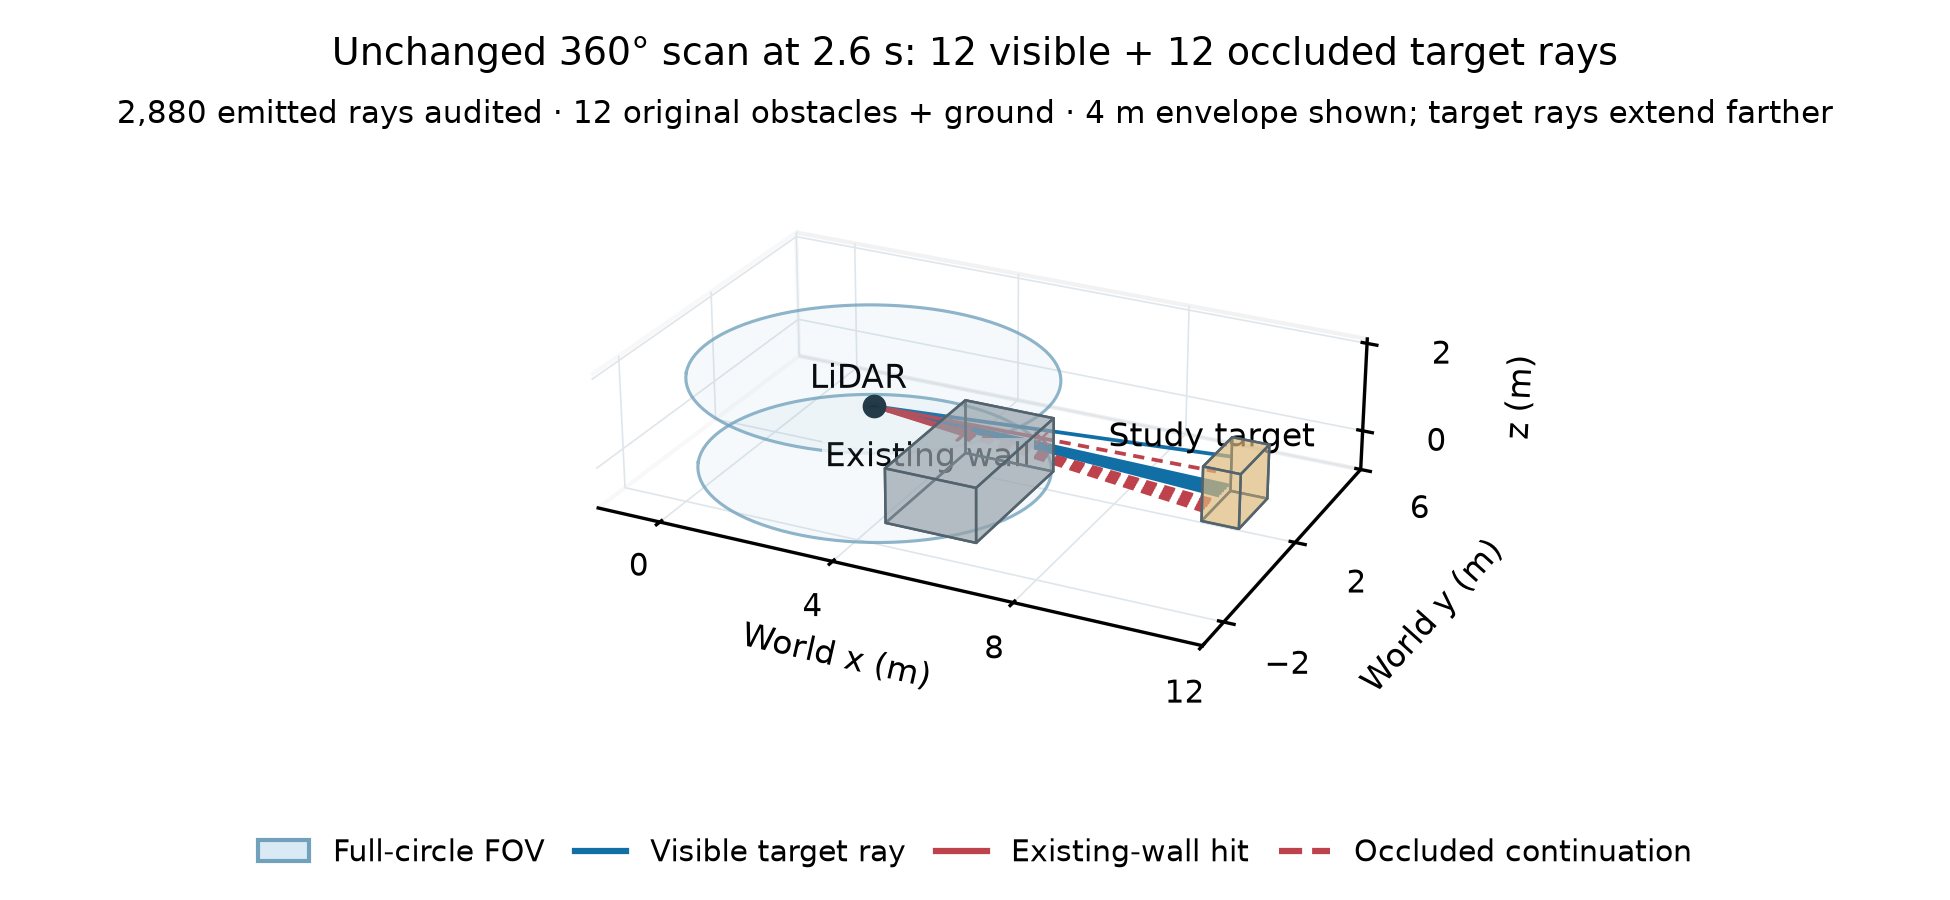
\includegraphics[width=0.86\linewidth,height=0.78in,keepaspectratio]{figures/weather_fov_los.png}
\caption{Baseline visibility at 2.6~s. The scan emits 2,880 rays; 12 hit the target and 12 target-directed rays are blocked by an existing wall. The drawing illustrates visibility, not measured points.}\label{fig:fov}
\end{figure}
\begin{figure}[H]\centering
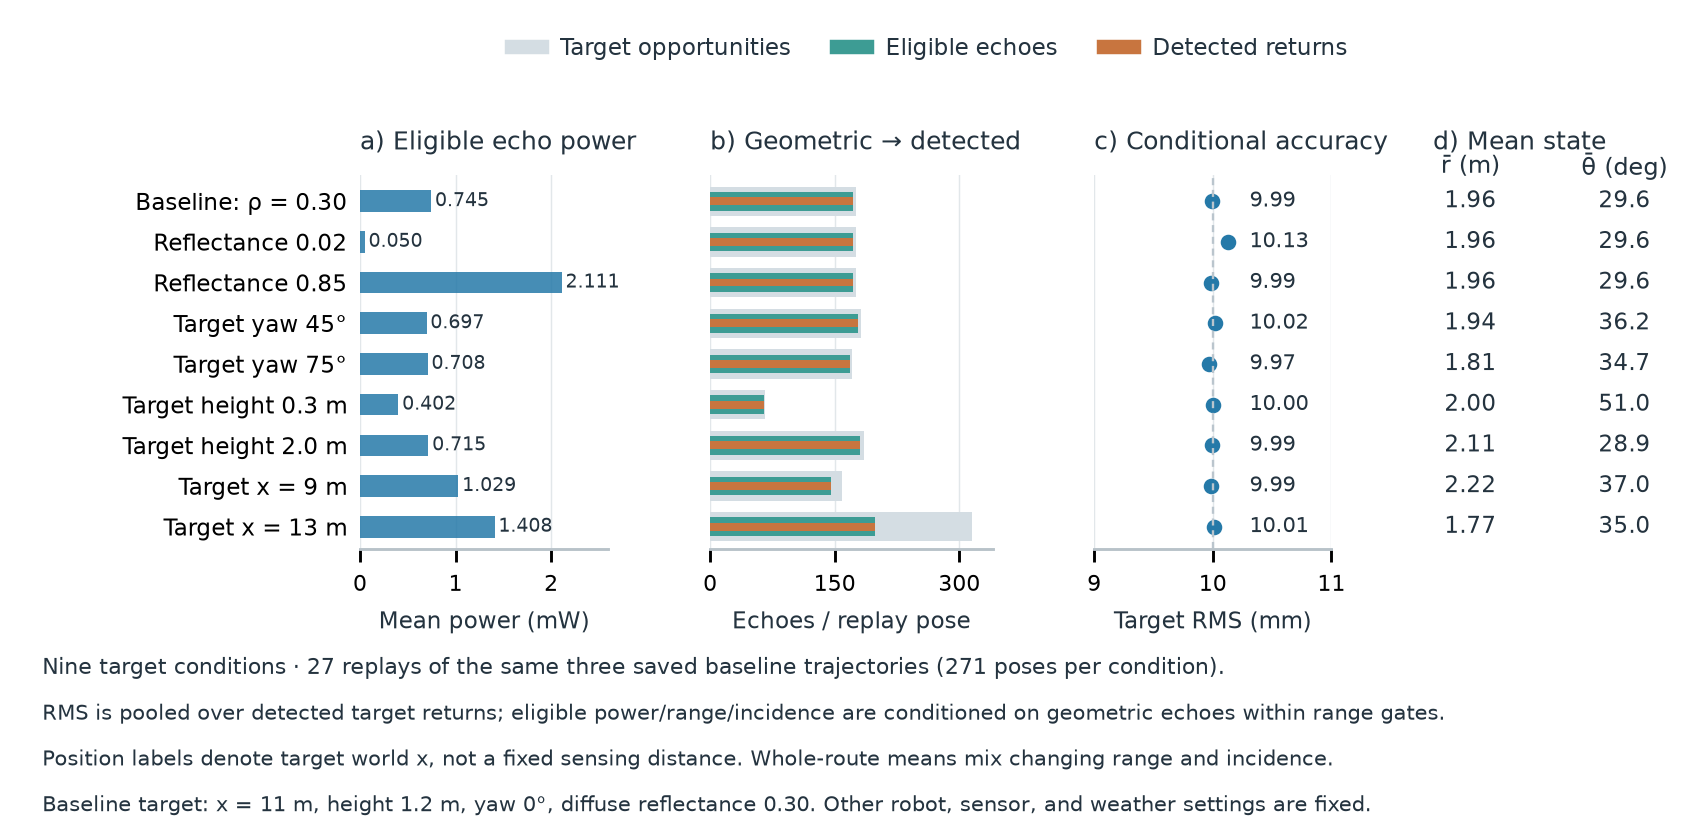
\includegraphics[width=0.90\linewidth,height=1.18in,keepaspectratio]{figures/target_characteristics.png}
\caption{Nine target settings replayed at the same baseline poses. Intersection, eligibility, and detection counts are separated; range RMS uses detected target returns only.}\label{fig:targets}
\end{figure}
Diffuse coefficients $0.02$, $0.30$, and $0.85$ produce $0.0667$, $1$, and $2.8333$ times baseline power. At 6~s in seed 1, target centers $x=9$, 11, and 13~m give ranges of 2.134, 4.011, and 5.950~m and powers of 0.339830, 0.105144, and 0.048696~mW, consistent with inverse-square spreading. Across the route, pose and visibility also affect the counts.

\begin{figure}[H]\centering
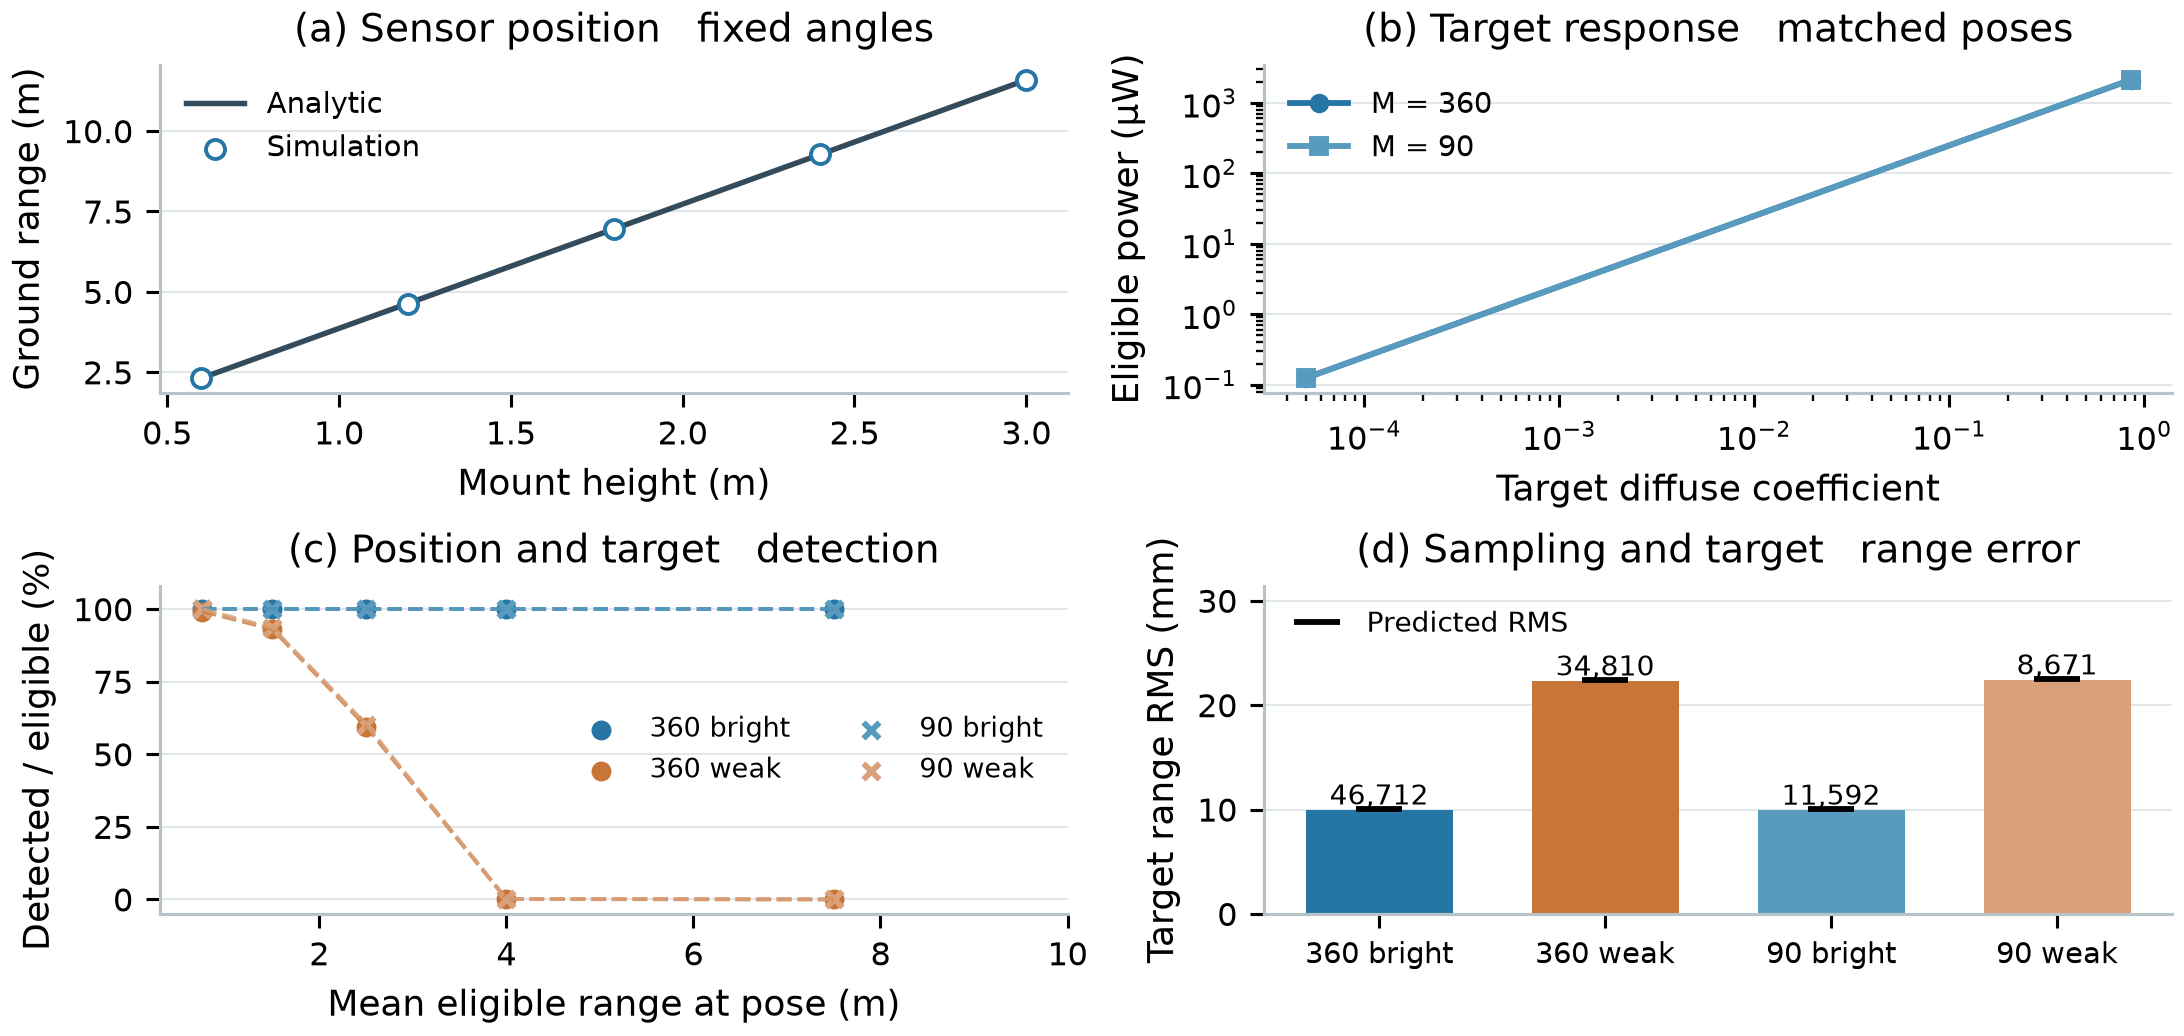
\includegraphics[width=0.88\linewidth,height=1.08in,keepaspectratio]{figures/sensor_dependencies.png}
\caption{Sensor mounting-height and sampling/reflectance comparisons. Slant range is measured along the beam to its ground intersection; the four factorial cases use matched poses.}\label{fig:sensor}
\end{figure}
At $-15^\circ$ elevation, raising the sensor from 0.6 to 3.0~m increases slant range from 2.318 to 11.591~m (Equation~\eqref{eq:height}). In the $80^\circ$ partial FOV, yaw angles of $0^\circ$, $40^\circ$, $45^\circ$, and $50^\circ$ yield 132, 70, 6, and 0 returns; the full-circle scan retains 132. This sharp edge effect comes from discrete beam geometry, not general detection probability.

The bright-to-weak coefficient ratio is 17,000. Increasing sampling from 90 to 360 azimuths raises bright-target detections from 11,592 to 46,712, although the grids do not hit identical points. At dense sampling, the weak target gives 34,810 detections (74.52\% of bright) and conditional RMS rises from 9.99 to 22.34~mm. With receiver noise raised tenfold, scene returns fall from 2,198.4 to 2,011.2 per scan but target RMS changes only from 9.992 to 10.082~mm; the strong baseline target means RMS alone can hide missed points.

\clearpage
\subsection{Weather measurements and detector validation}
\begin{figure}[H]\centering
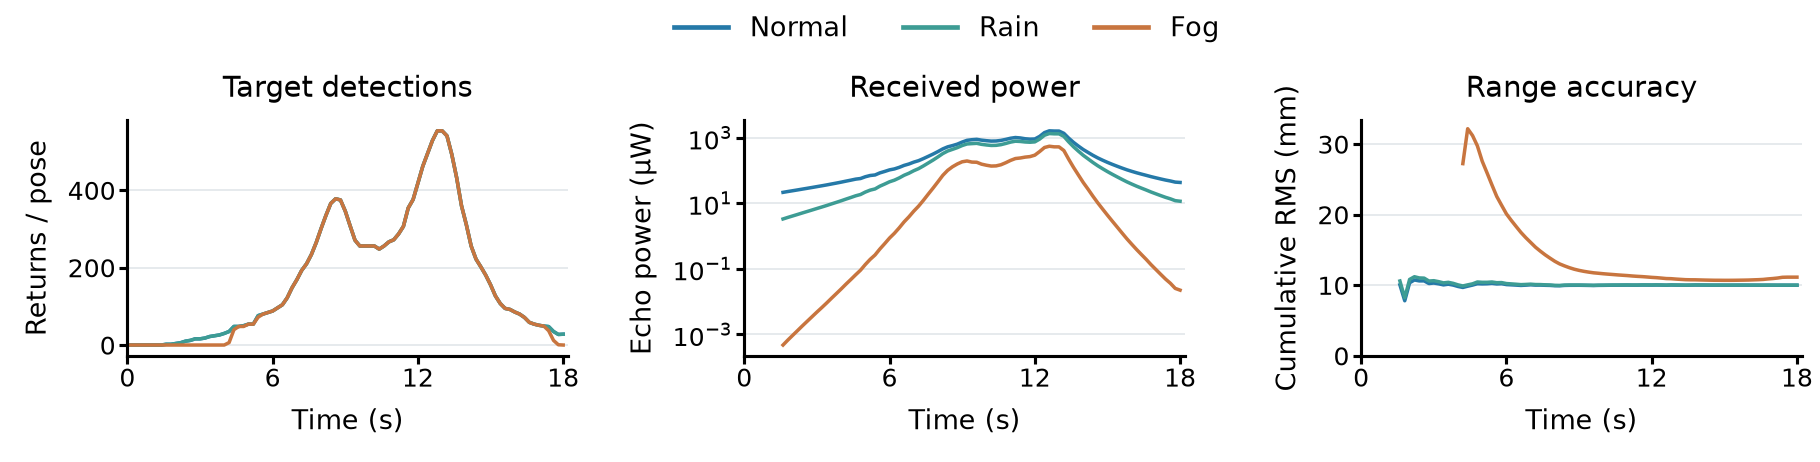
\includegraphics[width=0.88\linewidth,height=1.10in,keepaspectratio]{figures/weather_measurements_compact.png}
\caption{Normal-air, rain, and fog measurements replayed at matched baseline poses. Attenuation lowers received power; range RMS uses detected returns only.}\label{fig:weather}
\end{figure}
\begin{figure}[H]\centering
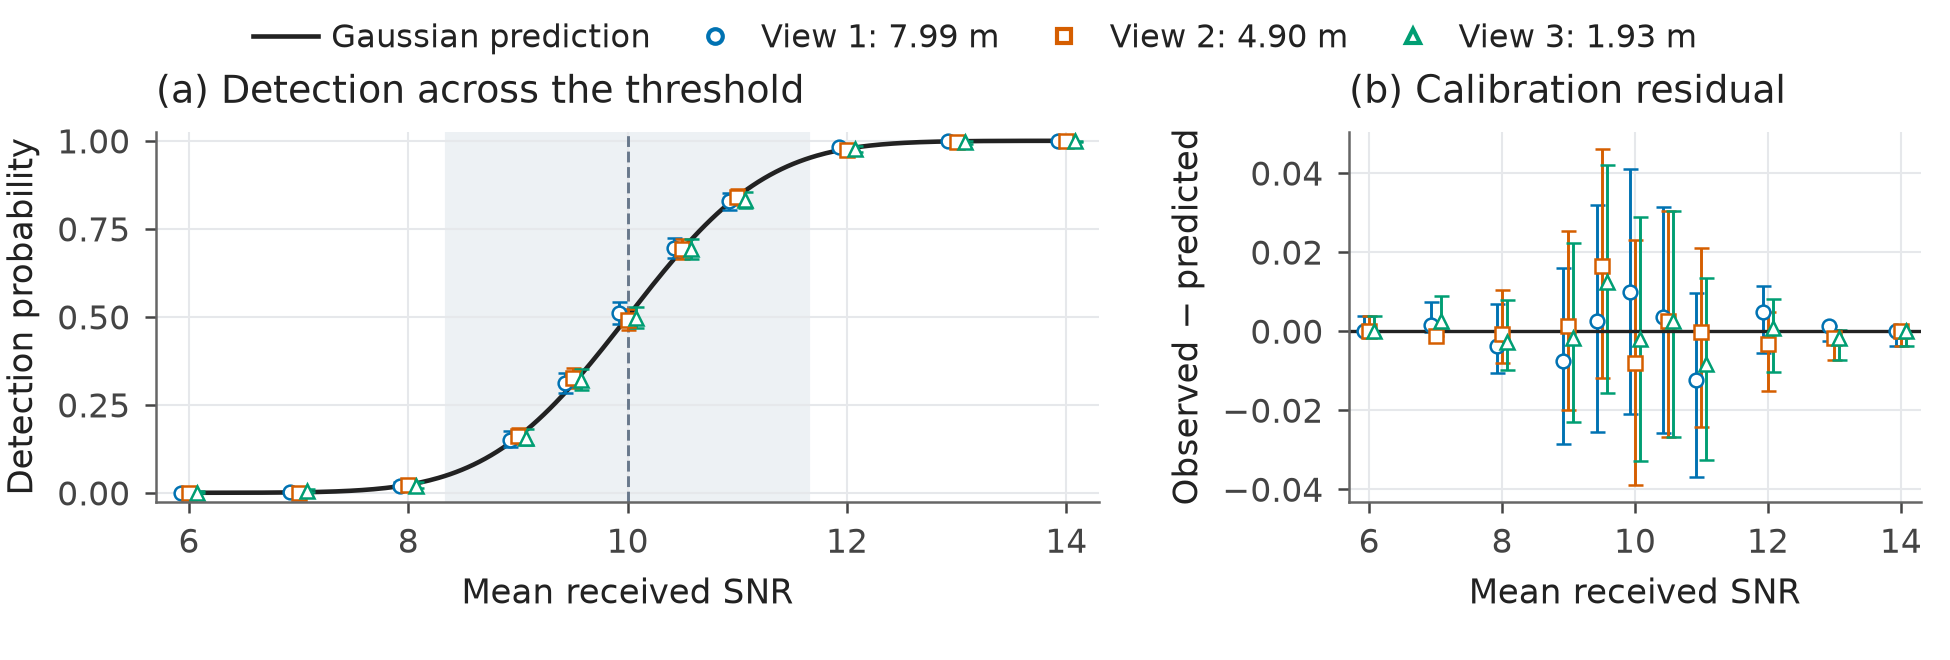
\includegraphics[width=0.88\linewidth,height=1.18in,keepaspectratio]{figures/report_threshold_detection.png}
\caption{Detection probabilities and residuals from 33,000 sensor trials. Each point summarizes 1,000 trials including misses; bars are pointwise 95\% Wilson intervals. The shaded band is the predicted 5--95\% transition range.}\label{fig:threshold}
\end{figure}
Weather replays retain high target-detection rates, so the separate threshold study tests the model where detection is uncertain. Three eligible rays at 7.99, 4.90, and 1.93~m were tested at 11 mean-SNR settings from 6 to 14, with 1,000 scans per setting. At mean SNR 10, the predicted probability is 0.5 and the observed fractions are 0.510, 0.492, and 0.498. Across 33 settings, detection-probability calibration RMS error is 0.547 percentage points, the maximum residual is 1.646 points, and 32 of 33 pointwise intervals contain the prediction. These intervals are pointwise, not simultaneous. For an observed fraction $\widehat p$ from $n$ trials, the Wilson interval is
\begin{equation}\label{eq:wilson}
\begin{aligned}
&\frac{\widehat p+\frac{a^2}{2n}\pm a\sqrt{\frac{\widehat p(1-\widehat p)}{n}+\frac{a^2}{4n^2}}}{1+\frac{a^2}{n}},\\[-2pt]
&\hspace{1em} a=1.96.
\end{aligned}
\end{equation}

In a separate 54,000-trial, 54-bin response study, the maximum probability residual is 0.032 and 52 of 54 intervals contain the prediction. Range-noise validation with 27,371 detections gives an observed RMSE of 30.869~mm versus 30.874~mm predicted; the standardized-error standard deviation is 1.00024, and 94.93\% of errors fall within $\pm1.96$. For detected echoes, define range error $e_i$, standardized error $\epsilon_i$, and RMSE as
\begin{equation}\label{eq:range_metrics}
\begin{aligned}
e_i&=z_i-r_{\mathrm{true},i},\qquad \epsilon_i=\frac{e_i}{\sigma_r(S_i)},\\
\mathrm{RMSE}&=\sqrt{\frac{1}{N_D}\sum_{i=1}^{N_D}e_i^2}.
\end{aligned}
\end{equation}
Across the current 16,507 detections, range RMS is 32.358~mm, compared with 32.287~mm predicted from conditional variance; standardized RMS is 1.0018. These checks support consistency with the implemented detector and noise assumptions, not the physical accuracy of a LiDAR device.

\clearpage
\subsection{Closed-loop weather runs and endpoint maps}
\begin{figure}[H]\centering
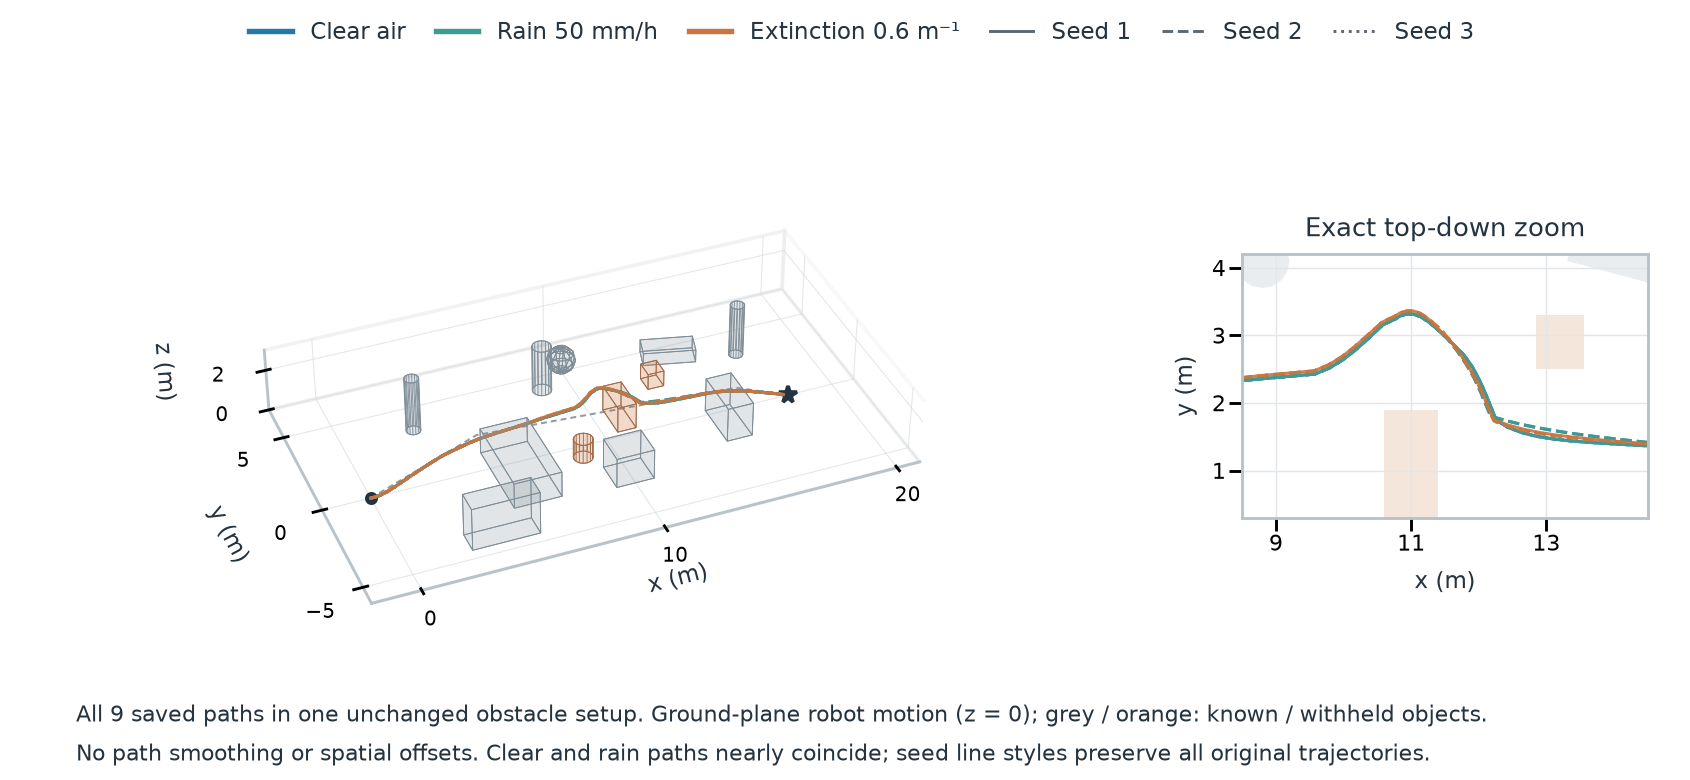
\includegraphics[width=0.87\linewidth,height=0.98in,keepaspectratio]{figures/weather_trajectories.png}\par\vspace{1pt}
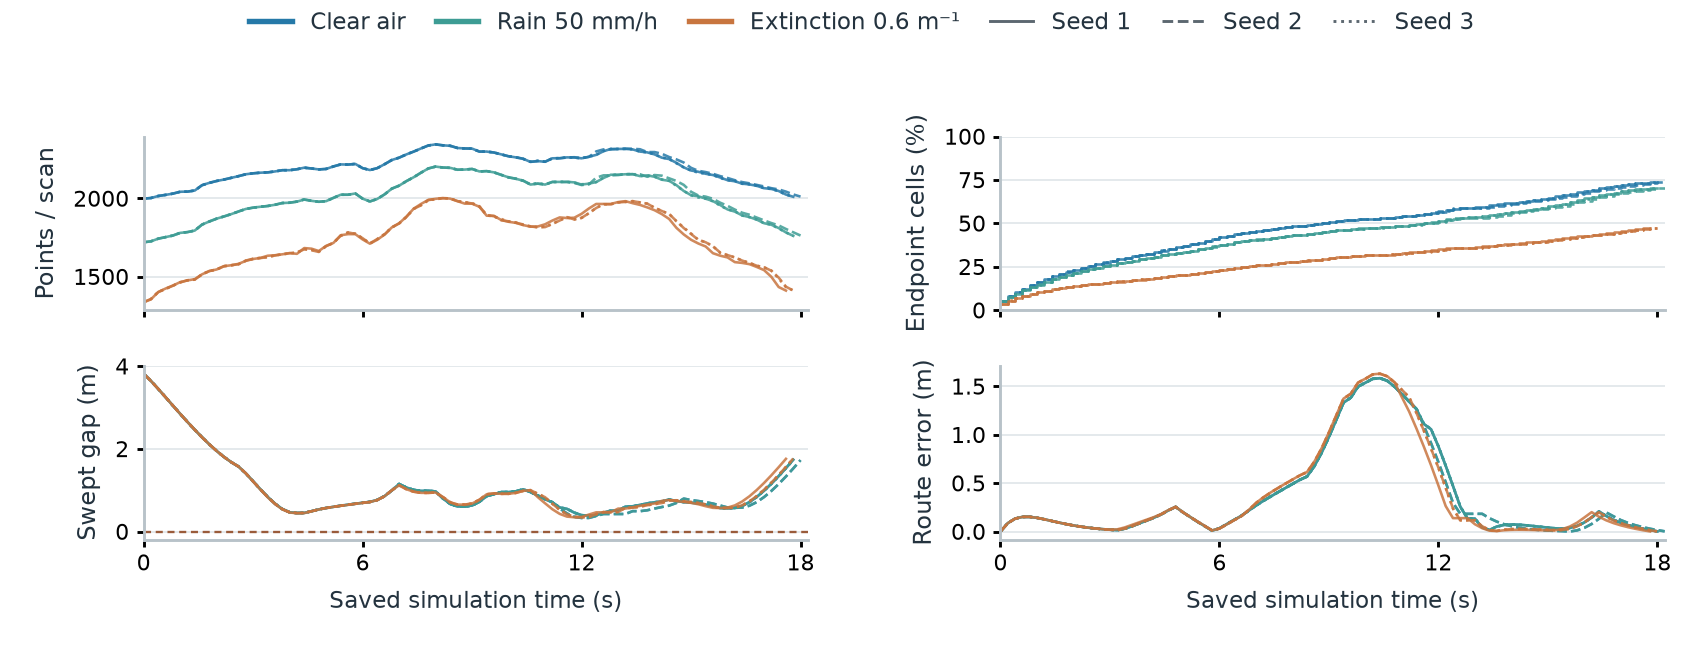
\includegraphics[width=0.87\linewidth,height=0.78in,keepaspectratio]{figures/weather_profiles.png}
\caption{Closed-loop trajectories and measurement profiles for all nine weather runs.}\label{fig:navigation}
\end{figure}
\begin{table}[H]\centering
\caption{Three-seed weather summary, except pooled target RMS and worst gap. All nine runs reached the goal.}\label{tab:weather}
{\footnotesize\setlength{\tabcolsep}{3.5pt}
\begin{tabular}{@{}lrrrrrrr@{}}\toprule
Condition & Points/scan & Map (\%) & RMS (mm) & Goals & Time (s) & Path (m) & Gap (m)\\\midrule
Normal & 2,198.4 & 73.67 & 9.992 & 3/3 & 18.07 & 19.702 & 0.330\\
Rain & 2,011.3 & 70.33 & 10.006 & 3/3 & 18.07 & 19.702 & 0.330\\
Fog & 1,742.0 & 47.10 & 11.139 & 3/3 & 17.93 & 19.784 & 0.345\\\bottomrule
\end{tabular}}
\end{table}
\begin{figure}[H]\centering
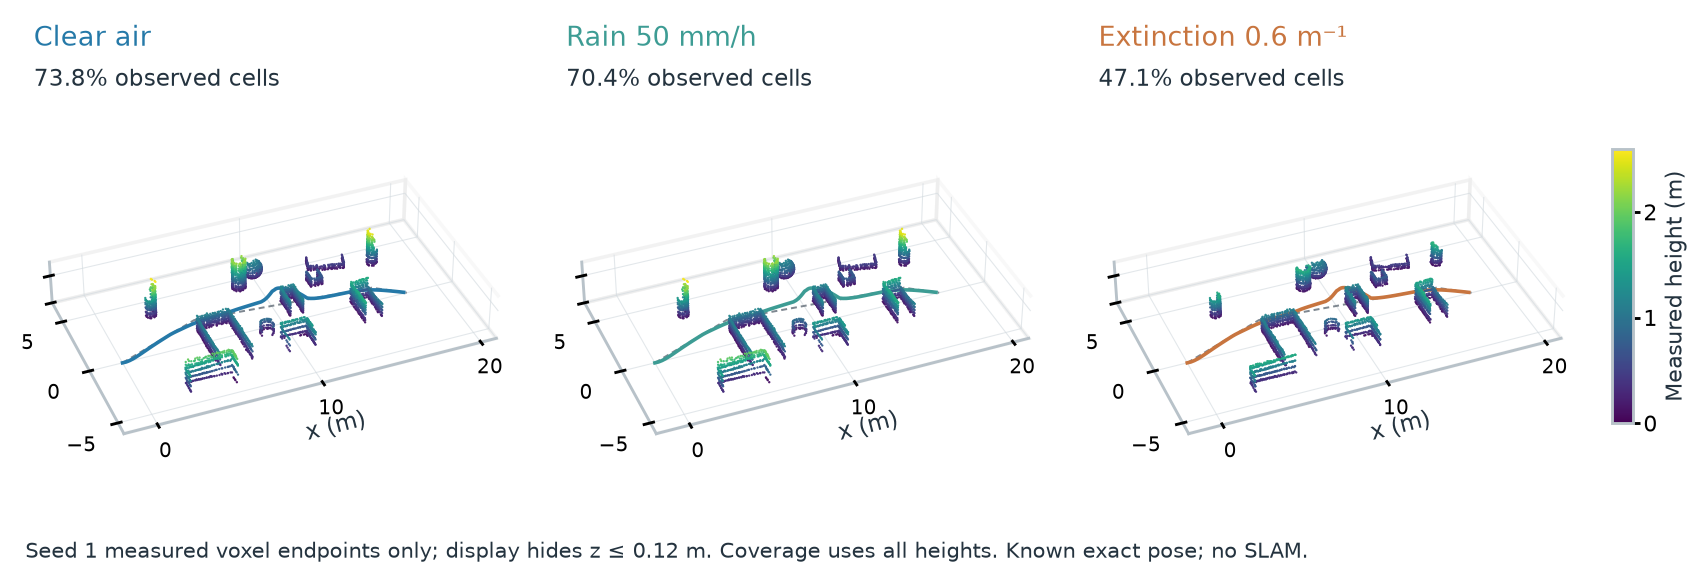
\includegraphics[width=0.87\linewidth,height=0.56in,keepaspectratio]{figures/weather_maps.png}
\caption{Seed-1 endpoint observations only, not free-space evidence; points below $z=0.12$~m are hidden.}\label{fig:maps}
\end{figure}
All nine runs reached the goal without collision or timeout. Mean returns per control step fall from 2,198.4 in normal air to 2,011.3 in rain and 1,742.0 in fog; fog produces 20.8\% fewer returns than normal air. Endpoint coverage falls from 73.67\% to 70.33\% in rain and 47.10\% in fog, a 26.57-point normal-to-fog decrease. Mean path length changes from 19.702 to 19.784~m, and the worst swept gap remains positive at 0.330--0.345~m. Three seeds in one static scene do not establish general safety.

Maps use $0.12$~m voxels and $0.2$~m endpoint cells over $[-2,21]\times[-6,7]$~m ($N_{\mathrm{ROI}}=7{,}475$). For a path with $K$ intervals, path length and observed-cell fraction are
\begin{equation}\label{eq:map}
\mathcal L=\sum_{k=0}^{K-1}\|\mathbf p_{k+1}-\mathbf p_k\|,\qquad f_{\mathrm{obs}}=\frac{N_{\mathrm{obs}}}{N_{\mathrm{ROI}}},\quad k=0,\ldots,K-1.
\end{equation}
\section{Conclusions}\label{sec:conclusion}
Analytic checks and repeated trials support the simulator's geometry, power, detection, and range-noise calculations. Denser sampling adds returns, weak echoes have larger conditional range error, and fog lowers coverage to 47.10\%. All nine runs completed the fixed route, but this is not a general safety result. Future work includes physical calibration, backscatter and scan-motion modeling, pose uncertainty, and broader scene tests.

\clearpage
\begin{thebibliography}{2}
\setstretch{1.0}\setlength{\itemsep}{2pt}
\bibitem{assignment} ``Midterm project,'' \emph{Robot Perception}, course assignment handout, pp.~1--2.
\bibitem{heiden} E.~Heiden, Z.~Liu, R.~K.~Ramachandran, and G.~S.~Sukhatme, ``Physics-based Simulation of Continuous-Wave LIDAR for Localization, Calibration and Tracking,'' in \emph{Proc. IEEE Int. Conf. Robot. Autom. (ICRA)}, 2020, pp.~2595--2601.
\end{thebibliography}
\end{document}
